\documentclass{article}
\usepackage{geometry}
\usepackage{listings}
\usepackage{textcomp}
\usepackage{graphicx}
\usepackage[hidelinks]{hyperref}
\usepackage{hyperref}
\usepackage{appendix}
\usepackage{multirow}
\usepackage{amsmath,amssymb,amsfonts}
\usepackage[framed,numbered,autolinebreaks,useliterate]{mcode}
%记得用xelatex
% 导入首行缩进用的宏包
\usepackage{indentfirst}
\setlength{\parindent}{2em}
% 每行缩进两个汉字
\usepackage{url}
\setlength{\parindent}{0pt}
\setlength{\parskip}{18pt}
\title{\vspace{+4cm}\textbf{First Applied Mathematics Assignment}}
\author{Jianqi Feng 202023092020}
\date{\today}
% //////////////////////////////////////////////////

\begin{document}
%标题
\maketitle
%目录
\newpage
\pagenumbering{Roman}
\setcounter{page}{0}
\tableofcontents

\newpage
\setcounter{page}{1}
\pagenumbering{arabic}


\section{Newton's Method}
\subsection{Nonlinear root-finding problem}
\setlength{\parindent}{2em}For the function $ f \in C^{2}[a,b]$ , consider the first Taylor polynomial for $f(x)$ expanded about $x_0$\cite{ref1} ,then we have the formula as follows.

\begin{align}
f(x) = f(x_0) + (x-x_0)f^{'}(x_0) + \frac{(x-x_0)^2}{2}f^{''}(\varsigma(x))
\label{taylor1}
\end{align}

Where $\varsigma(x)$ lies between $x$ and $x_0$.When $x_0$ is close to the approximation $p$ of $f(x)$,the $|x_0-p|$ is small , the term involving $(p-x_0)^2$ is much smaller,then we substantiate $p$ into (\ref{taylor1}), get the formula as follows.

\begin{align}
0 \approx f(x_0) + (p-x_0)f^{'}(x_0) \nonumber
\end{align}

Solving for p gives

\begin{align}
p\approx x_0 - \frac{f(x_0)}{f^{'}(x_0)}
\end{align}

When we starts with an initial approximation $p_0$ and generates the sequence $\left\{ p_n \right\}_{n=0}^{\infty}$,by

\begin{align}
p_n = p_{n-1} - \frac{f(p_{n-1})}{f^{'}(p_{n-1})} ,\quad \text{for} \enspace n=1.2.3……
\label{taylor2}
\end{align}

\subsection{For Example 1 $f(x) = cos(x)-x$}

According to the (\ref{taylor2}) , we could get the code in newton.mlx of the example 1 in Matlab as follows.

\begin{lstlisting}
% Part1 Newton's Method
% Nonlinear root-finding problem
clc;clear;
format long ;

%% example 1 f(x) = cos(x)-x
% step 1 set up the function
syms t ;
f = @(t) cos(t) - t ;
df = diff( f , t ) ; % calculate derivative of function f

% step 2 draw the figure to find the general result
a  = 0 ; b = pi/2 ; % input the interval of the root-finding 
m = linspace( a , b , 100 ) ; 
n = f(m) ;
plot( m , n ) ; % draw the figure
grid on ;
title('Figure To Find The Root (e.g.1)') ;
xlabel('x') ; 
ylabel('f(x)-x') ;

% step 3 find and input the general root
k = 10 ; % number of overlaps
x = zeros( 1 , k ) ;
x(1) = pi/4; % input the general root
for i = 2 : k
    x(i) = x(i-1) - f( x(i-1) )/subs( df, t ,x(i-1) );
end
x'  % plot the roots
\end{lstlisting}

In the step 2 ,we get the figure \ref{newton1} to find the general result

\begin{figure}[h!]
\centering
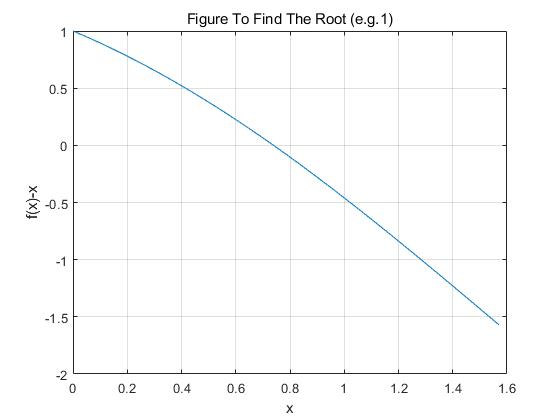
\includegraphics[width=0.6\textwidth]{newton.jpg}
\caption{Newton e.g.1}
\label{newton1}
\end{figure}

Then we input the general root $\frac{\pi}{4}$ into the program and get the sequence as follows:


\begin{table}[h!]
\centering
\begin{center}
 \begin{tabular}{c c} 
 \hline
 \hline
n & $p_n$ \\\hline
0 & 0.785398163397448\\ \hline
1 & 0.739536133515238\\ \hline
2 & 0.739085178106010\\ \hline
3 & 0.739085133215161\\ \hline
4 & 0.739085133215161\\ 
\hline
\hline
\end{tabular}
\end{center}
\caption{Sequence of e.g.1}
\label{newton table1}
\end{table}

The analysis before shows that the root is approximately equal to $p_3=0.739085133215161$.
Then we try another example to text the code.


\subsection{For Example 2 $f(x) = cos^3(x)-x$}
Change the function in the newton.mlx and we get the code as follows.


\begin{lstlisting}
%% example 2 f(x) = cos^3(x)-x
clc;clear;
format long ;
% step 1 set up the function
syms t ;
f = @(t) cos(t).^3 - t ;
df = diff( f , t ) ; % calculate derivative of function f

% step 2 draw the figure to find the general result
a  = 0 ; b = pi/2 ; % input the interval of the root-finding 
m = linspace( a , b , 100 ) ; 
n = f(m) ;
plot( m , n ) ; % draw the figure
grid on ;
title('Figure To Find The Root (e.g.2)') ;
xlabel('x') ; 
ylabel('f(x)-x') ;

% step 3 find and input the general root
k = 10 ; % number of overlaps
x = zeros( 1 , k ) ;
x(1) = pi/5; % input the general root
for i = 2 : k
    x(i) = x(i-1) - f( x(i-1) )/subs( df, t ,x(i-1) );
end
x'  % plot the roots
\end{lstlisting}

Same as the example ,in the step 2 ,we get the figure \ref{newton2} to find the general result

\begin{figure}[h!]
\centering
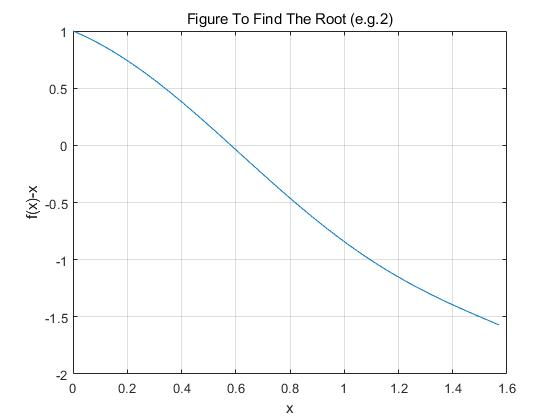
\includegraphics[width=0.6\textwidth]{newton2.jpg}
\caption{Newton e.g.2}
\label{newton2}
\end{figure}

Then we input the general root $\frac{\pi}{5}$ into the program and get the sequence as follows:


\begin{table}[h!]
\centering
\begin{center}
 \begin{tabular}{c c} 
 \hline
 \hline
n & $p_n$ \\\hline
0 & 0.628318530717959\\ \hline
1 & 0.582448516983119\\ \hline
2 & 0.582440071162041\\ \hline
3 & 0.582440071158208\\ \hline
4 & 0.582440071158208\\ 
\hline
\hline
\end{tabular}
\end{center}
\caption{Sequence of e.g.2}
\end{table}

The analysis before shows that the root is approximately equal to $p_3=0.582440071158208$.But the newton method will be in wrong situation when $p_0$ is not sufficiently close to the actual root,there is little reason to suspect that Newton's method will converge to the root.



\section{Steffensen's Method}
\subsection{Accelerating a normal fixed point iteration}
When we consider the $\left\{ p_n \right\}_{n=0}^{\infty}$,when that $n$ is sufficiently large\cite{ref1} we could say that

\begin{align}
\frac{p_{n+1}-p}{p_n-p}\approx \frac{p_{n+2}-p}{p_{n+1}-p} \nonumber
\end{align}

Then solving for p gives
\begin{align}
p\approx \frac{p_{n+2}p_n-p^2_{n+1}}{p_{n+2}-2p_{n+1}+p_n}
\label{Steffensen}
\end{align}

According to the (\ref{Steffensen}) which we remember as $\Delta^2$ ,when given the start $p_0$ we could get the value as follows:

\begin{align}
p^{(0)}_{0}\quad\quad\quad, \quad p^{(0)}_{1} = f(p^{(0)}_{0}), \quad p^{(0)}_{2} = f(p^{(0)}_{1})\nonumber\\
\nonumber\\
p^{(1)}_{0} = \Delta^2(p^{(0)}_{0}), \quad p^{(1)}_{1} = f(p^{(1)}_{0}), \quad p^{(1)}_{2} = f(p^{(1)}_{1})\nonumber
\end{align}

\subsection{Code Implementation of the Example}

According to the (\ref{Steffensen}), write the code in Matlab and get the result.

\begin{lstlisting}
%% example 1 x^3+4*x^2-10=0
clc;clear;
syms t ;
g = @(t) ( 10 / (t+4) ) ^ 0.5 ;%set up the function
k = 4 ;
p = zeros( 3 , k ) ; % The first to third lines are p_0,p_1,p_2
p(1,1) = 1.5 ;
p(2,1) = g( p(1,1) ) ;
p(3,1) = g( p(2,1) ) ;
for i = 2 : k
    p(1,i) = p(1,i-1) - ( p(2,i-1) - p(1,i-1) )^2/( p(3,i-1) - 2*p(2,i-1) + p(1,i-1) ) ;
    p(2,i) = g( p(1,i) ) ;
    p(3,i) = g( p(2,i) ) ;
end
p' % show the result
\end{lstlisting}

Then we get the values as follows

\begin{table}[h!]
\centering
\begin{center}
 \begin{tabular}{c c c c} 
 \hline
 \hline
$k$ & $p^{(k)}_{0}$ & $p^{(k)}_{1}$  & $p^{(k)}_{2}$\\ \hline
0 & 1.500000000000000 &1.348399724926484 &1.367376371991283\\ 
1 & 1.365265223957260 &1.365225533619792 &1.365230583376005\\ 
2 & 1.365230013416586 &1.365230013413780 &1.365230013414137\\ 
3 & 1.365230013414097 &1.365230013414097 &1.365230013414097\\ 
\hline
\hline
\end{tabular}
\end{center}
\caption{Sequence of Steffensen's Method}
\end{table}

It appears that Steffensen's method gives quadratic convergence without evaluating a derivative.
Then we compared Steffensen's method with the Newton's method.

\subsection{Compared with the Newton's method}

Use the same example and we compare the sequence of the two methods.Here are the code in Matlab.

\begin{lstlisting}
%% compared with the newton's method
clc;clear;
format long ;
% step 1 set up the function
syms t ;
f = @(t) ( 10 / (t+4) ) ^ 0.5 - t ;
df = diff( f , t ) ; % calculate derivative of function f

% step 2 find and input the general root
k = 10 ; % number of overlaps
x = zeros( 1 , k ) ;
x(1) = 1.5; % input the general root
for i = 2 : k
    x(i) = x(i-1) - f( x(i-1) )/subs( df, t ,x(i-1) );
end
x'  % plot the roots
% Obviously this method converges faster
\end{lstlisting}

\begin{table}[h!]
\centering
\begin{center}
 \begin{tabular}{c c c c c} 
 \hline
 \hline
  & \multicolumn{3}{c}{Steffensen's method} & Newton's method \\ \hline
$k$ & $p^{(k)}_{0}$ & $p^{(k)}_{1}$  & $p^{(k)}_{2}$ & $p_n$\\ \hline\hline
0 & 1.500000000000000 &1.348399724926484 &1.367376371991283 &1.500000000000000\\ 
1 & 1.365265223957260 &1.365225533619792 &1.365230583376005 &1.364953916057443\\ 
2 & 1.365230013416586 &1.365230013413780 &1.365230013414137 &1.365230012211262\\ 
3 & 1.365230013414097 &1.365230013414097 &1.365230013414097 &1.365230013414097\\ 
\hline
\hline
\end{tabular}
\end{center}
\caption{Sequence of Steffensen's Method}
\end{table}

Then we get the sequence as shown above,obviously Steffensen's method converges faster.The number of iterations when solving with the Steffensen iteration method is much smaller, which shows that the Steffensen iterative method accelerates the convergence rate.

\section{M$\ddot u$ller's method}

\subsection{Finding all zeros of a polynomial}
We consider the quadratic polynomial as follows at first

\begin{align}
P(x) = a(x-x_2)^2+b(x-x_2)+c \nonumber
\end{align}

that passes through 3 points $(x_0,f(x_0))$,$(x_1,f(x_1))$,$(x_2,f(x_2))$.Then we can substantiate those points into the polynomial shown above,and get the equations as follows.

\begin{equation}
    \begin{cases}
        f(x_0) = a(x_0-x_2)^2 + b(x_0-x_2) + c \\
        f(x_1) = a(x_1-x_2)^2 + b(x_1-x_2) + c\\ 
        f(x_2) = a \cdot 0^2 + b \cdot 0 + c = c
     \end{cases}
\end{equation}

Next solve the equation for $a$,$b$ and $c$ , we can get the result as follows:

% \begin{align}
% a = \frac{1}{x_0-x_1} \left( \frac{f(x_0)-f(x_2)}{x_0-x_2}-\frac{f(x_1)-f(x_2)}{x_1-x_2} \right) \nonumber 
% \end{align}

% \begin{align}
% b = \frac{1}{x_0-x_1} \left[ \frac{(x_0-x_2)(f(x_1)-f(x_2))}{x_1-x_2} - \frac{(x_1-x_2)(f(x_0)-f(x_2))}{x_0-x_2}\right] \nonumber
% \end{align}

% \begin{align}
% c = f(x_2) \nonumber
% \end{align}

\begin{equation}
    \begin{cases}
        a = \frac{1}{x_0-x_1} \left( \frac{f(x_0)-f(x_2)}{x_0-x_2}-\frac{f(x_1)-f(x_2)}{x_1-x_2} \right) \\
        b = \frac{1}{x_0-x_1} \left[ \frac{(x_0-x_2)(f(x_1)-f(x_2))}{x_1-x_2} - \frac{(x_1-x_2)(f(x_0)-f(x_2))}{x_0-x_2}\right]\\ 
        c = f(x_2)
        \label{solve}
     \end{cases}
\end{equation}

We know that $x_2$ and $x_3$ which we need to find out both are the roots of $f(x)=0$.According to the Veda's theorem\cite{ref2} we can get the result of $x_3$ with less roundoff error problems.

\begin{align}
x_3 = x_2 - \frac{2c}{b+sgn(b)\sqrt{b^2-4ac}} \nonumber
\end{align}

\subsection{M$\ddot u$ller's method in Matlab}
Accoeding to the (\ref{solve}) , to make $x_3$ close to $x_2$ enough,we choose the larger $|b+sgn(b)\sqrt{b^2-4ac}|$\cite{ref1} and get the code in Matlab as follows

\begin{lstlisting}
%Part3 Muller's method
%Finding all zeros of a polynomial(including comples roots)
function y=muller(x_0,x_1,x_2,tol)
syms x ;
f = @(x) 16*x^4 - 40*x^3 + 5*x^2 + 20*x +6 ;%set up the function
x0 = x_0 ; % input the value x_0
x1 = x_1 ; % input the value x_1
x2 = x_2 ; % input the value x_2
TOL = tol;
h = 1;
i = 1;
result=[];
while i<100
    h1 = x1 - x0 ;
    h2 = x2 - x1 ;
    e1 = ( f( x1 ) - f( x0 ) ) / h1 ;
    e2 = ( f( x2 ) - f( x1 ) ) / h2 ;
    d = ( e2 - e1 ) / ( h2 + h1 ) ;
    b = e2 + h2 * d ;
    D = (b*b - 4*f(x2)*d)^0.5 ;
    a = ( abs(b-D) < abs(b+D) ) ;
    E = a*(b+D) + (1-a)*(b-D) ;
    h = -2*f(x2) / E ;
    if abs(h) < TOL
        break;
    else
    p = x2 + h ;
    % next step
    x0 = x1 ;
    x1 = x2 ;
    x2 = p ;
    result = [result;[ x2 , f(x2) , h]];
    i = i+1;
    end
end
y = result ;
end
\end{lstlisting}

Then we can get the results of the different 3 points that given to us by calling the function-muller.m.Here are some examples.

\begin{lstlisting}
% if we change the value of x_0,x_1,x_2
% xi f(xi) TOL from left to right
muller(0.5,-0.5,0,10^-5)
muller(0.5,1.0,1.5,10^-5)
muller(2.5,2.0,2.25,10^-5)
\end{lstlisting}

\begin{table}[h!]
\begin{center}
\caption{when $x_0 = 0.5 ,\quad x_1 = -0.5 ,\quad x_2 = 0$}
 \begin{tabular}{c c c c} 
 \hline
 \hline
$k$ & $x_i$ & $f(x_i)$ & $TOL$\\ \hline
3 & -0.5555556+0.5983516i &-29.4007011-3.8987247i &-0.5555556+0.5983516i\\ 
4 & -0.4354503+0.1021012i &1.3322248-1.1930967i &0.1201053-0.4962504i\\ 
5 & -0.3906315+0.1418522i &0.3750579-0.6701684i &0.0448188+0.0397510i\\ 
6 & -0.3576984+0.1699263i &-0.1467501-0.0074462i &0.0329330+0.0280740i\\ 
7 & -0.3560507+0.1628560i &-0.0018402+0.0005385i &0.0016478-0.0070703i\\ 
8 & -0.3560617+0.1627583i &0.0000016+0.0000009i &-0.0000110-0.0000977i\\ 
\hline
\hline
\end{tabular}
\end{center}
\end{table}

% \begin{table}[h!]
% \begin{center}
%  \begin{tabular}{c c c c} 
%  \hline
%  \hline
% \multicolumn{4}{c}{$x_0 = 0.5 ,\quad x_1 = 1.0 ,\quad x_2 = 1.5$} \\
% $k$ & $x_i$ & $f(x_i)$ & $TOL$\\ \hline
% 3 & 1.287855 &-1.376275e+00 &-2.121453e-01\\ \hline
% 4 & 1.237459 &1.269454e-01 &-5.039599e-02\\ \hline
% 5 & 1.241605 &2.193409e-03 &4.145764e-03\\ \hline
% 6 & 1.241677 &-5.704036e-07 &7.294967e-05\\ \hline
% 7 & 1.241677 &-2.273737e-13 &-1.896606e-08\\ \hline
% \hline
% \hline
% \end{tabular}
% \end{center}
% \caption{when $x_0 = 0.5 ,\quad x_1 = 1.0 ,\quad x_2 = 1.5$}
% \end{table}

% \begin{table}[h!]
% \begin{center}
%  \begin{tabular}{c c c c} 
%  \hline
%  \hline
% \multicolumn{4}{c}{$x_0 = 2.5 ,\quad x_1 = 2.0 ,\quad x_2 = 2.25$} \\
% $k$ & $x_i$ & $f(x_i)$ & $TOL$\\ \hline
% 3 & 1.960592 &-6.113100e-01 &-2.894077e-01\\ \hline
% 4 & 1.970564 &7.455499e-03 &9.971314e-03\\ \hline
% 5 & 1.970447 &2.916094e-05 &-1.170635e-04\\ \hline
% 6 & 1.970446 &4.576606e-11 &-4.597920e-07\\ \hline
% \hline
% \hline
% \end{tabular}
% \end{center}
% \caption{when $x_0 = 2.5 ,\quad x_1 = 2.0 ,\quad x_2 = 2.25$}
% \end{table}

\begin{table}
\begin{minipage}[c]{0.48\textwidth}
\caption{when $x_0 = 0.5 ,\quad x_1 = 1.0 ,\quad x_2 = 1.5$}
\begin{tabular}{c c c c} 
 \hline
 \hline
$k$ & $x_i$ & $f(x_i)$ & $TOL$\\ \hline
3 & 1.287855 &-1.376275e+00 &-2.121453e-01\\ \hline
4 & 1.237459 &1.269454e-01 &-5.039599e-02\\ \hline
5 & 1.241605 &2.193409e-03 &4.145764e-03\\ \hline
6 & 1.241677 &-5.704036e-07 &7.294967e-05\\ \hline
7 & 1.241677 &-2.273737e-13 &-1.896606e-08\\ \hline
\hline
\end{tabular}
\end{minipage}
\begin{minipage}[c]{0.6\textwidth}
\centering
\caption{when $x_0 = 2.5 ,\quad x_1 = 2.0 ,\quad x_2 = 2.25$}
 \begin{tabular}{c c c c} 
 \hline
 \hline
$k$ & $x_i$ & $f(x_i)$ & $TOL$\\ \hline
3 & 1.960592 &-6.113100e-01 &-2.894077e-01\\ \hline
4 & 1.970564 &7.455499e-03 &9.971314e-03\\ \hline
5 & 1.970447 &2.916094e-05 &-1.170635e-04\\ \hline
6 & 1.970446 &4.576606e-11 &-4.597920e-07\\ \hline
\hline
\end{tabular}
\end{minipage}
\end{table}


The actual values for this equation are $1.241677,1.970446,$ and $-0.356062 \pm 0.1627558i$ ,which demonstrates the accuracy of the approximations from M$\ddot u$ller's method.

\newpage
\clearpage
\phantomsection
\addcontentsline{toc}{section}{References}
\tolerance=500
\begin{thebibliography}{99}  
\bibitem{ref1}Richard L. Burden, J. Douglas Faires, Annette M. Burden “Numerical Analysis” Cengage Learning, 2015
\bibitem{ref2}[J]Letters in Mathematical PhysicsVolume 39, Issue 4. 1997. PP 349-353 
\end{thebibliography}
\end{document}



